% --------------------------------------------------------------------------- %
% --------------------------------------------------------------------------- %
\chapter{The Large Hadron Collider and the CMS Detector}
\label{ch:detector}

In order to probe the most fundamental constituents of nature, accelerators ramp particles up to great energies and then collide them to probe particle interactions. Detectors situated at the collision point can measure the outgoing products from particle collisions, and physicists can study the interactions to measure SM parameters, determine particle properties, quantify interaction rates, or search for new particles and processes.

The Large Hadron Collider is the most powerful particle accelerator ever constructed, and collides protons at a rate of nearly one billion times per second at a record energy of 13 Teraelectronvolts. The Compact Muon Solenoid is one of the all-purpose physics detectors that monitors the products of proton-proton collisions delivered by the LHC. Together with the ATLAS detector (A Toroidal LHC ApparatuS), the CMS detector is responsible for collecting data to measure a wide range of physics phenomena.

% --------------------------------------------------------------------------- %
% --------------------------------------------------------------------------- %
\section{The Large Hadron Collider}
\label{sec:lhc}

% --------------------------------------------------------------------------- %
% --------------------------------------------------------------------------- %

% --------------------------------------------------------------------------- %
% --------------------------------------------------------------------------- %
\section{The Compact Muon Solenoid}
\label{sec:cms}
The Compact Muon Solenoid (CMS) is a general-purpose physics detector at the LHC, situated at one of the five collision points along the main ring. The detector encapsulates the collision point with layers of various subsystems designed to interact with the outgoing particles of the proton-proton collisions, and measure the position and energies of the collision products. Because of the extremely high rate of interactions at the collision point (on the order of one billion interactions per second), saving data from every bunch crossing would be unsustainable, and so the detector is also equipped with a system of hardware and software implemented "triggers" which identify events of interest for physics analyses to be saved to disk for further analysis.

The physical construction of the detector is motivated by the different interaction of particles with different types of materials, and consists of several subsystems layered as coaxial cylinders around the interaction point. Each subsystem consists of (sometimes different) components covering the fiducial area coaxial with the beamline (the {\it barrel}) and also the ends of the cylinder (the {\it endcap}). The innermost subsystem of CMS is the silicon tracker, which consists of many layered silicon pixels designed to pinpoint the locations of charged particles while minimally interacting with the particle's trajectory. The layer beyond the tracker is the electromagnetic calorimeter (ECAL), a grid of lead-tungstate crystals which scintillate to measure the energies of electromagnetic particles. Beyond the ECAL is the hadronic calorimeter (HCAL), a sampling calorimeter designed to measure the energies of hadronic particles (which deposit minimal energy in the ECAL). The final, outer layer is the CMS muon detector, where the muon detection stations are interweaved with the magnetic return yoke that generates the toroidal 3.8T magnetic field inside the detector volume. The total dimensions of the detector are 21.6m long and 14.6m in diameter, weighing over 12,500 tons.

\subsection{Silicon Tracker} 
\label{subsec:tracker}
The silicon vertex tracker (SVT) is a series of silicon pixels and strips designed to measure the position of charged particles in the detector, while disturbing their path as little as possible. The position of particles in the interior is of particular importance in event reconstruction; charged particles traveling in a magnetic field will deflect in a curved path with radius proportional to the particles momentum as described in equation \ref{eq:momentum}, and so the track reconstruct can be used to not only determine a particle's momentum with high precision, but also the sign of its charge based on the direction of curvature.
\begin{equation}
	\label{eq:momentum}
	p = qrB
\end{equation}
As the innermost detector subsystem, the SVT experiences the highest flux of particle radiation. In the barrel region, the tracker layers are oriented in 3 coaxial layers. Closest to the interaction point where particle flux is the greatest, very precise silicon pixels are used, measuring $100\times150 \mu \text{m}^2$, whereas in other layers the flux is low enough to use microstrip detectors, measuring $10 \text{cm}\times80\mu \text{m}$ and  $25 \text{cm}\times180\mu \text{m}$ in the middle and outer layers respectively. In the endcaps, the pixel strips are arranged in a turbine-like pattern in two separate layers on each end. This configuration allows for the precise measurement of particle position for track reconstruction, while minimizing the amount of material which might deflect particles from their original trajectories. A partial geometry of the SVT layout can be seen in figure \ref{fig:pixelLayout}.
\begin{figure}
	\centering
	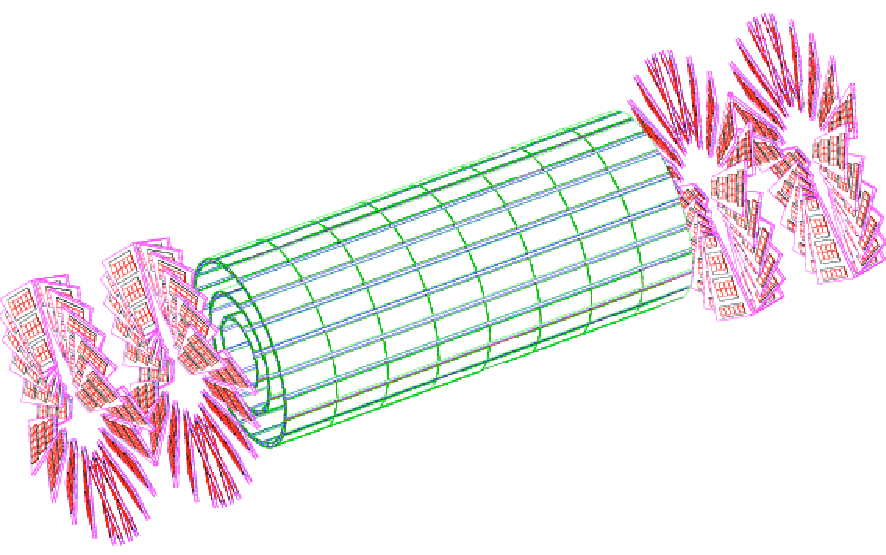
\includegraphics[width=0.95\textwidth]{detector/figs/trackerGeometry}
	\caption{Geometry of silicon tracker inner layers in CMS.}
	\label{fig:pixelLayout}
\end{figure}

\subsection{Electromagnetic Calorimeter}
\label{subsec:ecal}
The ECAL is used to measure the energies of particles which interact electromagnetically, both absorbing the incident particles and scintillating to provide an energy-readout to photodiodes attached to each crystal. Constructed of lead-tungstate ($\text{PbWO}_4$), electromagnetically interacting particles (such as electrons or photons) will interact with the crystal material, losing energy through a cascade of electromagnetic interactions including election-positron pair production and bremsstrahlung. This phenomenon --- also referred to as "showering" --- causes the crystals to scintillate proportional to the energy deposited in the crystal, which is then measured by various photodiodes to extract an accurate measurement of the particle energy, now fully absorbed by the calorimeter.
%\begin{figure}
%	\centering
%	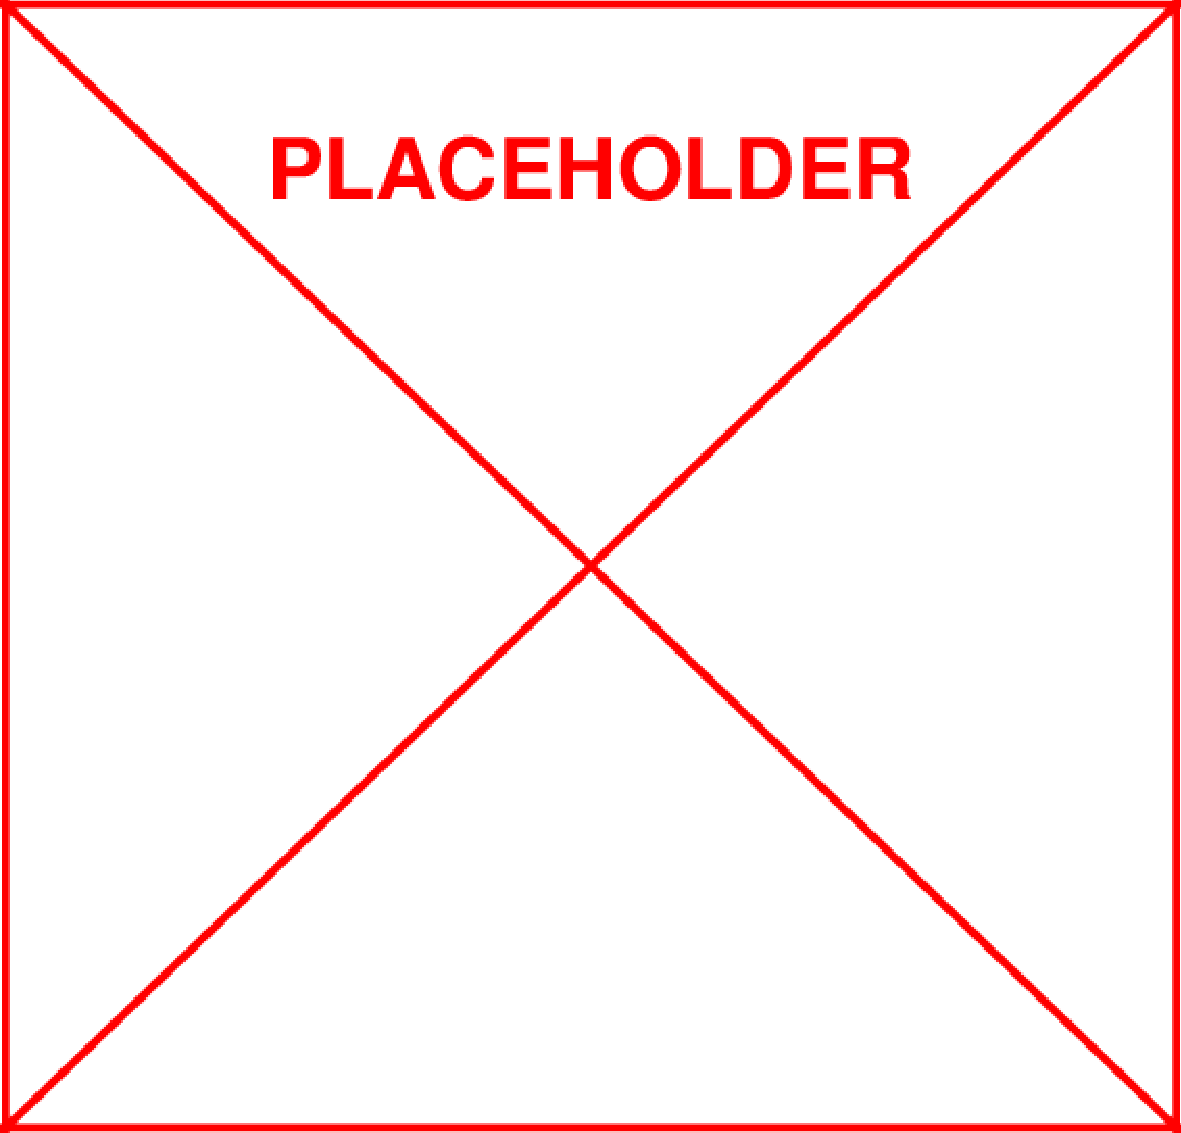
\includegraphics[width=0.4\textwidth]{figs/placeholder}
%	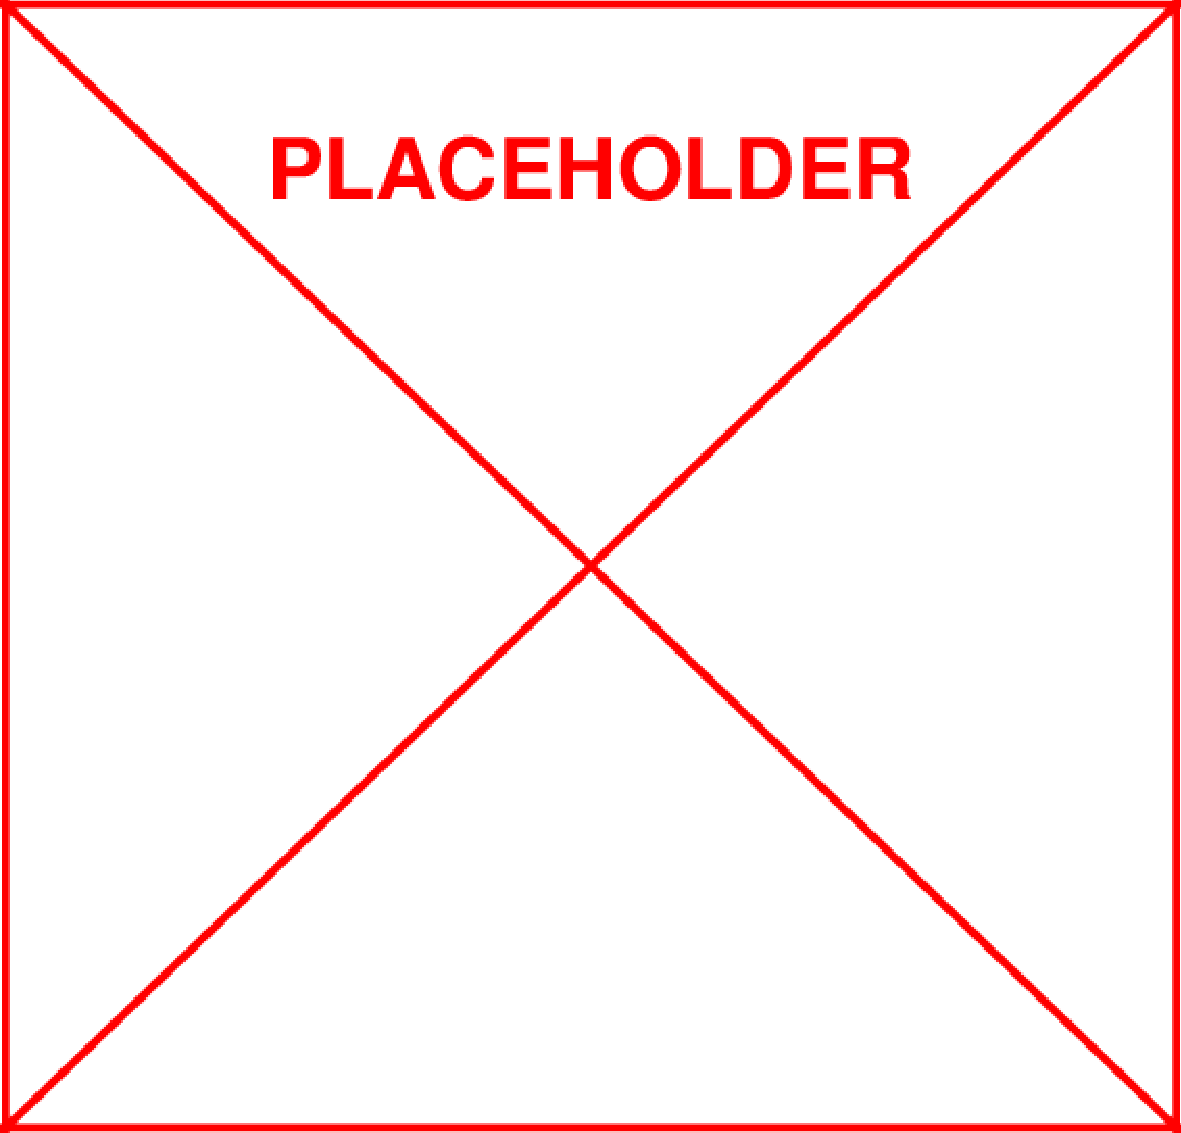
\includegraphics[width=0.4\textwidth]{figs/placeholder}
%	\caption{Feynman diagrams depicting the main processes by which particles shower in the ECAL. The left diagram depicts electron-positron pair production from a photon, and the right diagram depicts bremsstrahlung, where an electron radiates energy away through a photon.}
%	\label{fig:ecalFeynman}
%\end{figure}

The fundamental principle of the calorimeter measurement relies on the energy loss of particles interacting with matter. In general, the energy of a particle traveling a distance $X$ through some material is given by equation \ref{eq:energyDist}, where $E_0$ is the initial energy of the particle and $X_0$ is the material-dependent radiation length. 
\begin{equation}
	\label{eq:energyDist}
	E(x)=E_0 e^{\frac{-x}{X_0}}
\end{equation}
The design of the calorimeter is motivated by the choice of a scintillating, radiation-hard material with short $X_0$ such that incident electromagnetic particles deposit all their energy and are stopped by the ECAL. The resolution of the energy measurement is also dependent on the "stochastic term", which parametrizes the uncertainty due to statistical and measurement fluctuations in the calorimeter, and is given by equation \ref{eq:ecalSigma}, where $S$ is the stochastic term, $N$ the noise, and $C$ the constant term. 
\begin{equation}
	\label{eq:ecalSigma}
	\left(\frac{\sigma}{E}\right)^2=\left(\frac{S}{\sqrt{E}}\right)^2+\left(\frac{N}{E}\right)^2+C^2
\end{equation}
The energy resolution can be measured by a test beam of known energy, as shown in figure \ref{fig:ecalSigma}.
\begin{figure}
	\centering
	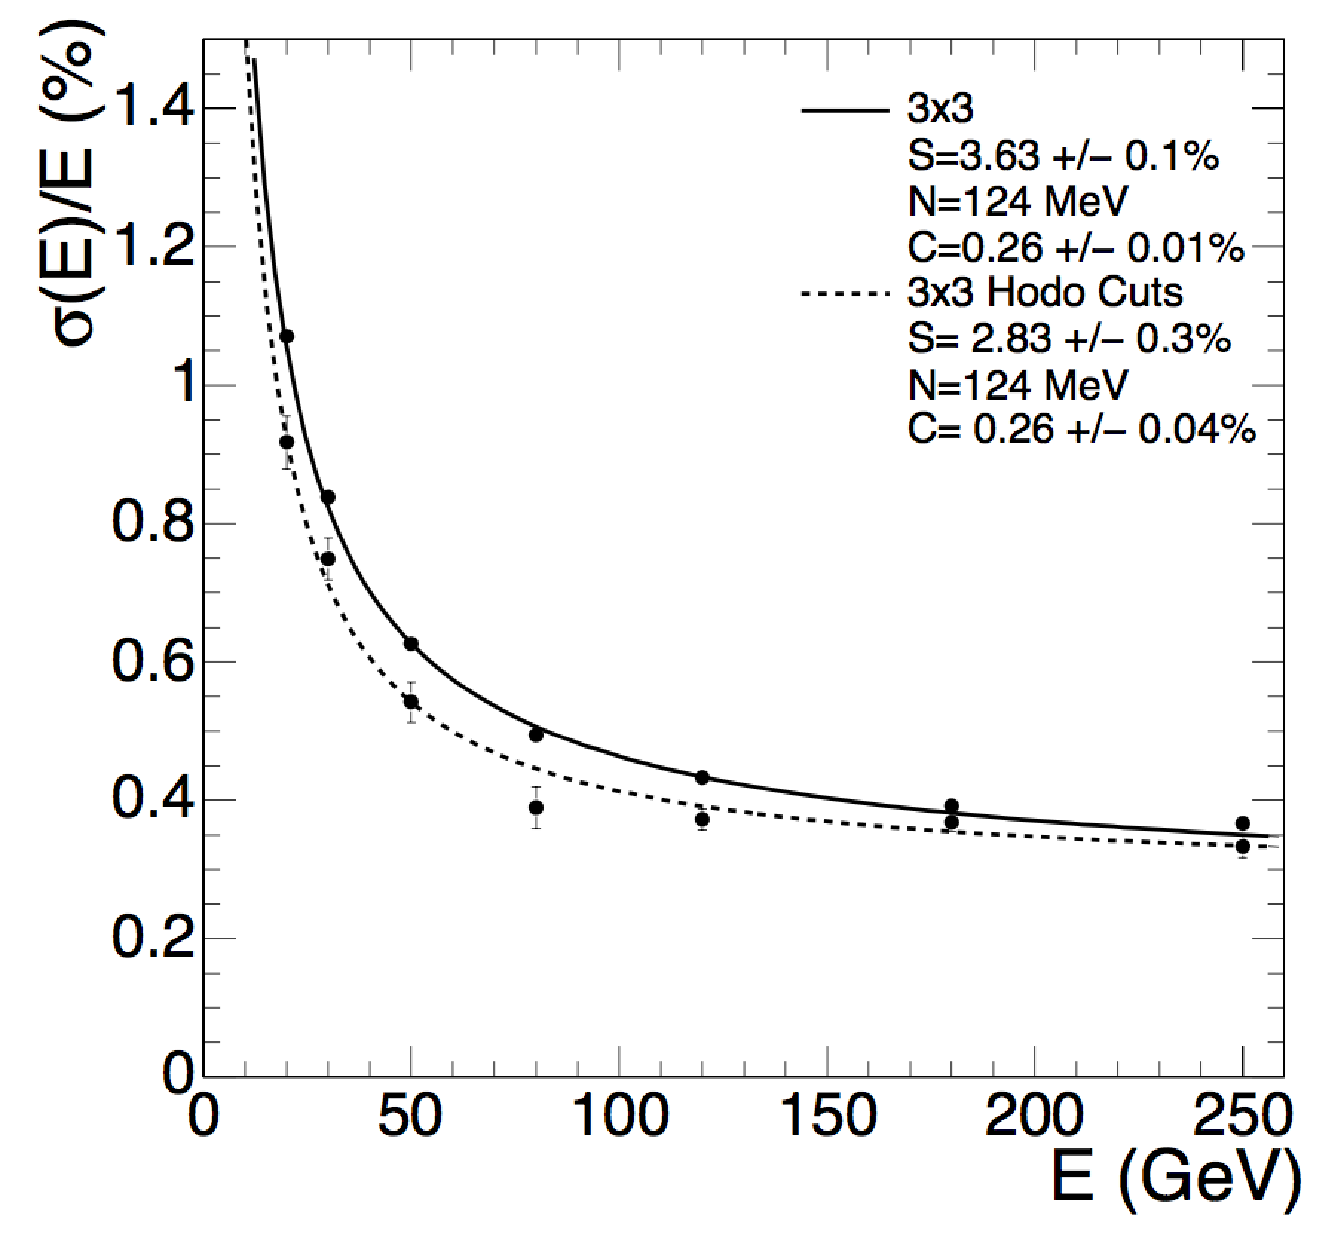
\includegraphics[width=0.65\textwidth]{detector/figs/ecalRes}
	\caption{Energy resolution $\sigma/E$ of the ECAL as a function of electron energy measured using a test beam. The energy was measured in a $3\times3$ crystal array with electrons incident on the center crystal, with electrons falling in a $4\times4\text{mm}^2$ region (lower points) and $20\times20\text{mm}^2$ region (upper points).}
	\label{fig:ecalSigma}
\end{figure}

The construction of the calorimeter is also divided into two sections by the cylindrical geometry, the ECAL barrel section (EB) and ECAL endcap sections (EE). The EB consists of 61,200 crystals arranged into 36 "supermodules", each spanning half the barrel length, and uses silicon avalanche photodiodes (APDs) as photodetectors. The individual crystals are tilted slightly (3\textdegree) in an $\eta-\phi$ grid with respect to the nominal interaction point, with a front-facing area of $22\times22\text{mm}^2$ and a length of 230mm. The EE instead uses vacuum phototriodes (VPTs) as photodetectors, and consists of approximately 15,000 crystals clustered in $5\times5$ units, also offset from the interaction point but arranged in an $x-y$ grid, with a cross section of $28.6\times28.6\text{mm}^2$ and a length of 220mm. The EE is also equipped with a "preshower" device placed in front of the crystal calorimeter, consisting of two strips of silicon strip detectors to enhance $\pi^0$ rejection. The layout of the ECAL can be seen in figure \ref{fig:ecalGeometry}. Because of the depth of the ECAL crystals (which are $\sim25X_0$, and the confining properties of the crystals (which have a Moliere radius of 2.2cm, the radius of a cylinder containing 90\% of a shower's energy on average), electrons and photons are typically well reconstructed in CMS, except in the transition region where EB and EE meet.
\begin{figure}
	\centering
	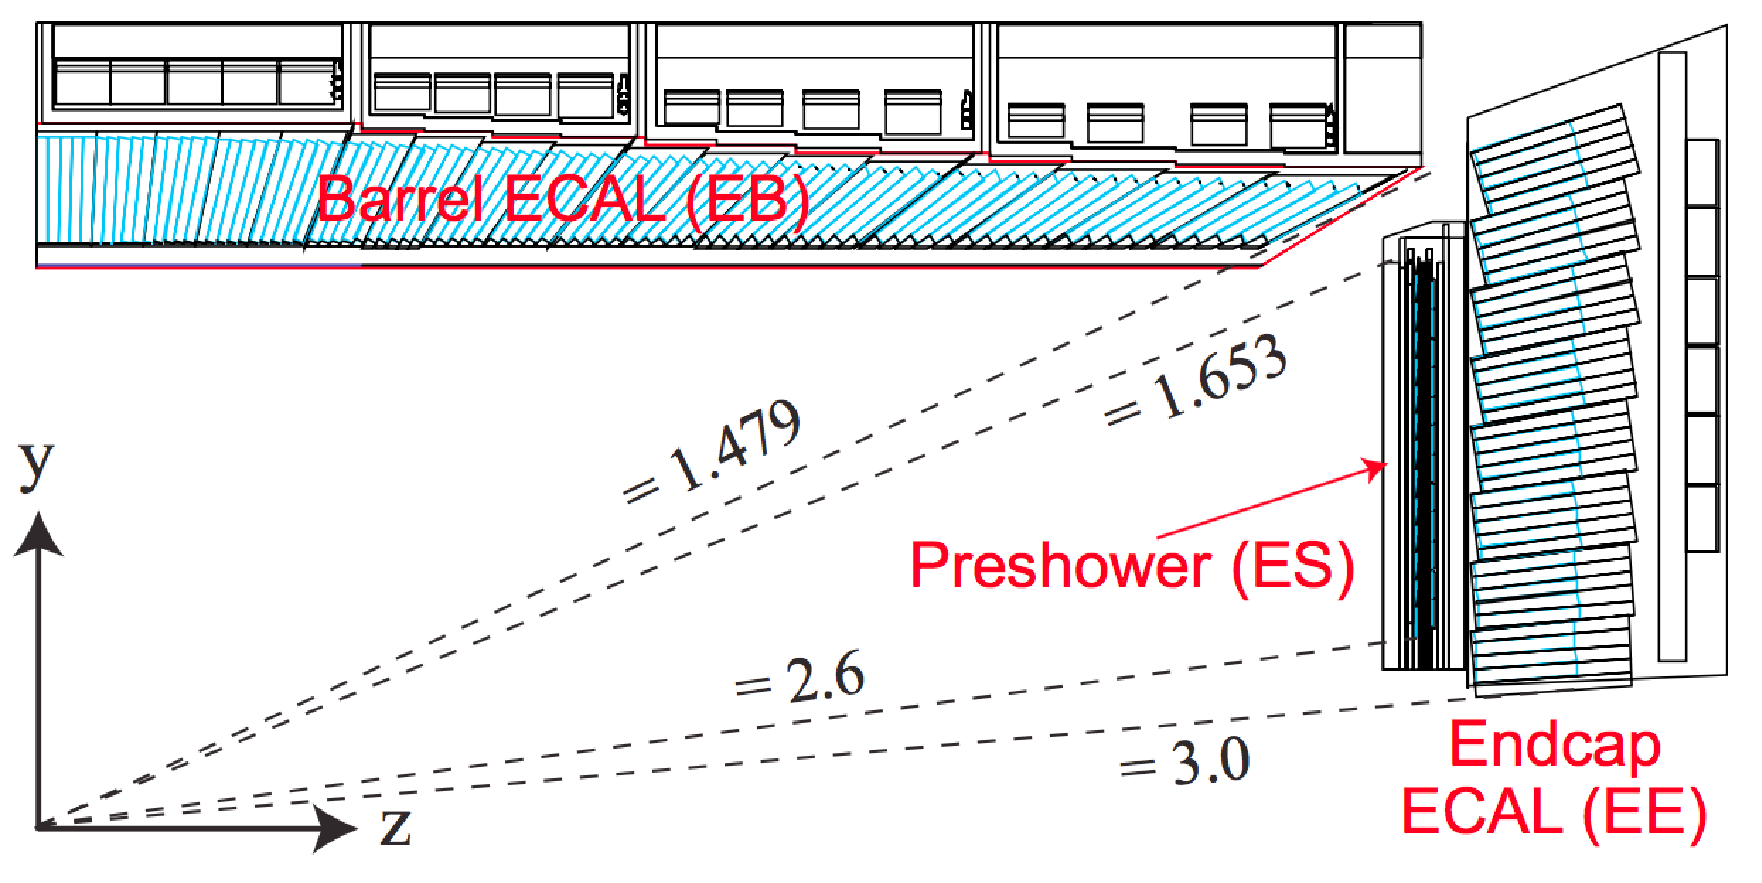
\includegraphics[width=0.95\textwidth]{detector/figs/ecalGeometry}
	\caption{A cross section of the ECAL geometry, with the dashed lines marking the pseudorapidity values $\eta$ covered by the various subsystems.}
	\label{fig:ecalGeometry}
\end{figure}

\subsection{Hadronic Calorimeter}
\label{subsec:hcal}
The CMS HCAL is a sampling calorimeter. Designed with alternating layers of scintillating and absorbing material, incident hadronic particles (such as charged pions, kaons, protons, etc.) interact with the absorber material and consequently shower into electromagnetic particles, whose energy can be read out by photodiodes connected to the scintillating material. Brass is used as the absorber material for both its interaction length and non-magnetic properties, and plastic scintillator tiles connected to embedded wavelength-shifting fibers carry the light to a readout system.

As with the ECAL, the energy loss of hadronic particles in the absorber is characterized by the (hadronic) interaction length and equation \ref{eq:energyDist}. However, unlike the ECAL, the HCAL contains both hadronic and electromagnetic showers. Electromagnetic particles generated in hadronic showers  often fail to escape the absorber layers, and thus some electromagnetic energy is lost in the absorbers. The CMS HCAL is sometimes referred to as a {\it non-compensating calorimeter} because it is not constructed to actively compensate for the energy lost to these electromagnetic effects and the energy measurements must be corrected offline, known as "jet energy corrections" (JECs).  JECs are typically calculated by examining data from collisions producing a boson recoiling against  hadronic particles. By accurately measuring the boson energy in the ECAL, the sum of the recoiling hadronic energy in the HCAL is inferred (by momentum conservation) and compared to the detector response. Because the performance of the HCAL can fluctuate with time and run conditions, JECs are regularly recalculated and applied to the raw energy measurements taken by the HCAL to compensate for these effects. Additional information on the corrections contained in JECs is detailed in section \ref{subsec:jets}. The energy resolution of the HCAL in different regions of pseudorapidity can be seen in figure \ref{fig:hcalSigma}.
 \begin{figure}
	\centering
	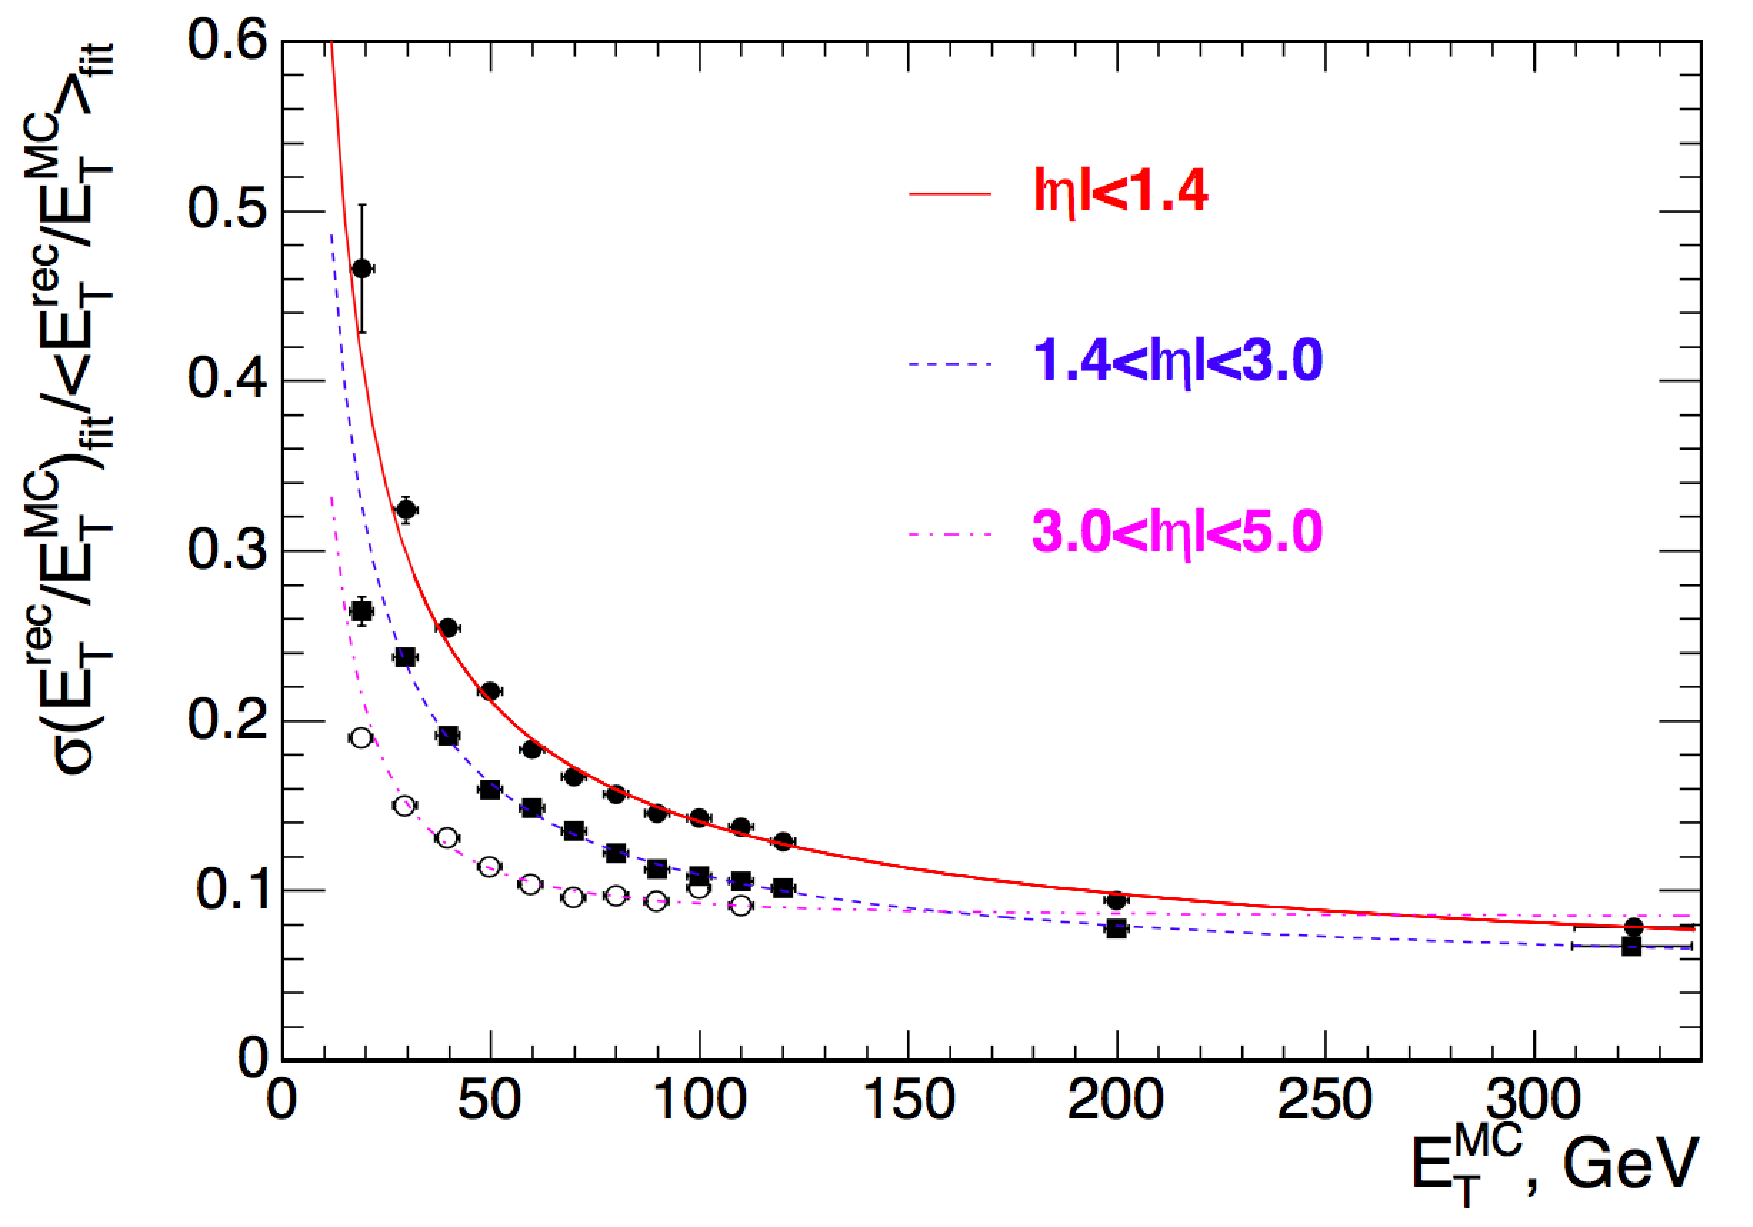
\includegraphics[width=0.75\textwidth]{detector/figs/jetEnergyRes}
	\caption{The jet transverse energy resolution as a function of the jet transverse energy, in different regions of pseudorapidity. For an explanation of jets, see section \ref{subsec:jets}}
	\label{fig:hcalSigma}
\end{figure}

The geometry of the HCAL can be reduced to four sections. The HCAL barrel (HB) consist of 32 "towers" of alternating absorber/scintillator material spanning the pseudorapidity region $-1.4<\eta<1.4$. The HCAL outer (HO) detector lies outside the vacuum tank of the magnetic coil and measures energy from any hadronic particles "leaking" through the HB, covering the pseudorapidity region $-1.26<\eta<1.26$. The HCAL endcap (HE) consists of 14 $\eta$ towers spanning the pseudorapidity range $1.3<|\eta|<3.0$. Finally, the HCAL forward (HF) is a different steel/quartz fibre calorimeter spanning the very-forward $3.0<|\eta|<5.0$ region. Instead utilizing Cherenkov radiation generated in the quartz fibers, the HF preferentially samples neutral hadronic energy and is ideally designed for the hadronic-heavy radiation environment in the forward region.

\subsection{Muon Detectors}
\label{subsec:muondetector}
The muon detector is the only subsystem which is constructed outside of the toroidal magnetic field. Interleaved with the magnetic return yoke, different muon detectors are used to aid in the identification and reconstruction of muon tracks. Because muons typically penetrate every other layer of the detector and have a large bending radius, additional measurements in the muon system --- combined with measurements in the SVT --- can lead to vastly improved resolution of muon momentum. The non-uniform magnetic field in the muon detector region (beyond the toroidal regime) causes an s-shaped trajectory and tighter bending radius (than in the SVT) for the muons, which improves the resolution for particles with transverse momentum above $\sim200\text{GeV}$ as seen in figure \ref{fig:muonSigma}.
 \begin{figure}
	\centering
	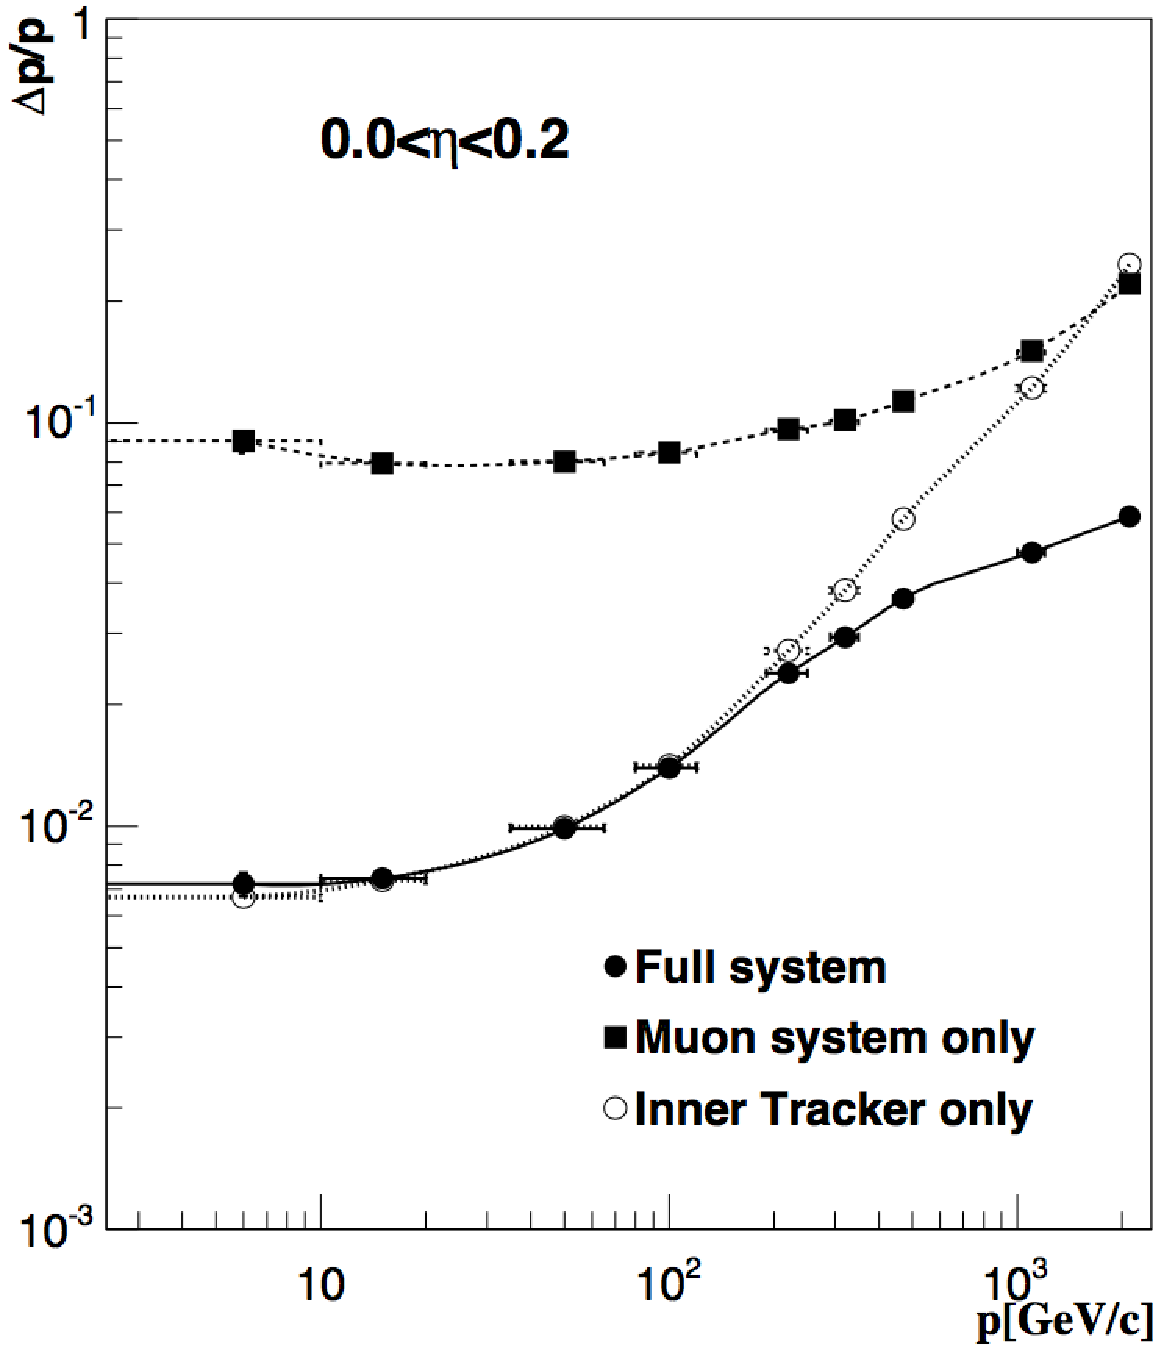
\includegraphics[width=0.45\textwidth]{detector/figs/muonResInner}
	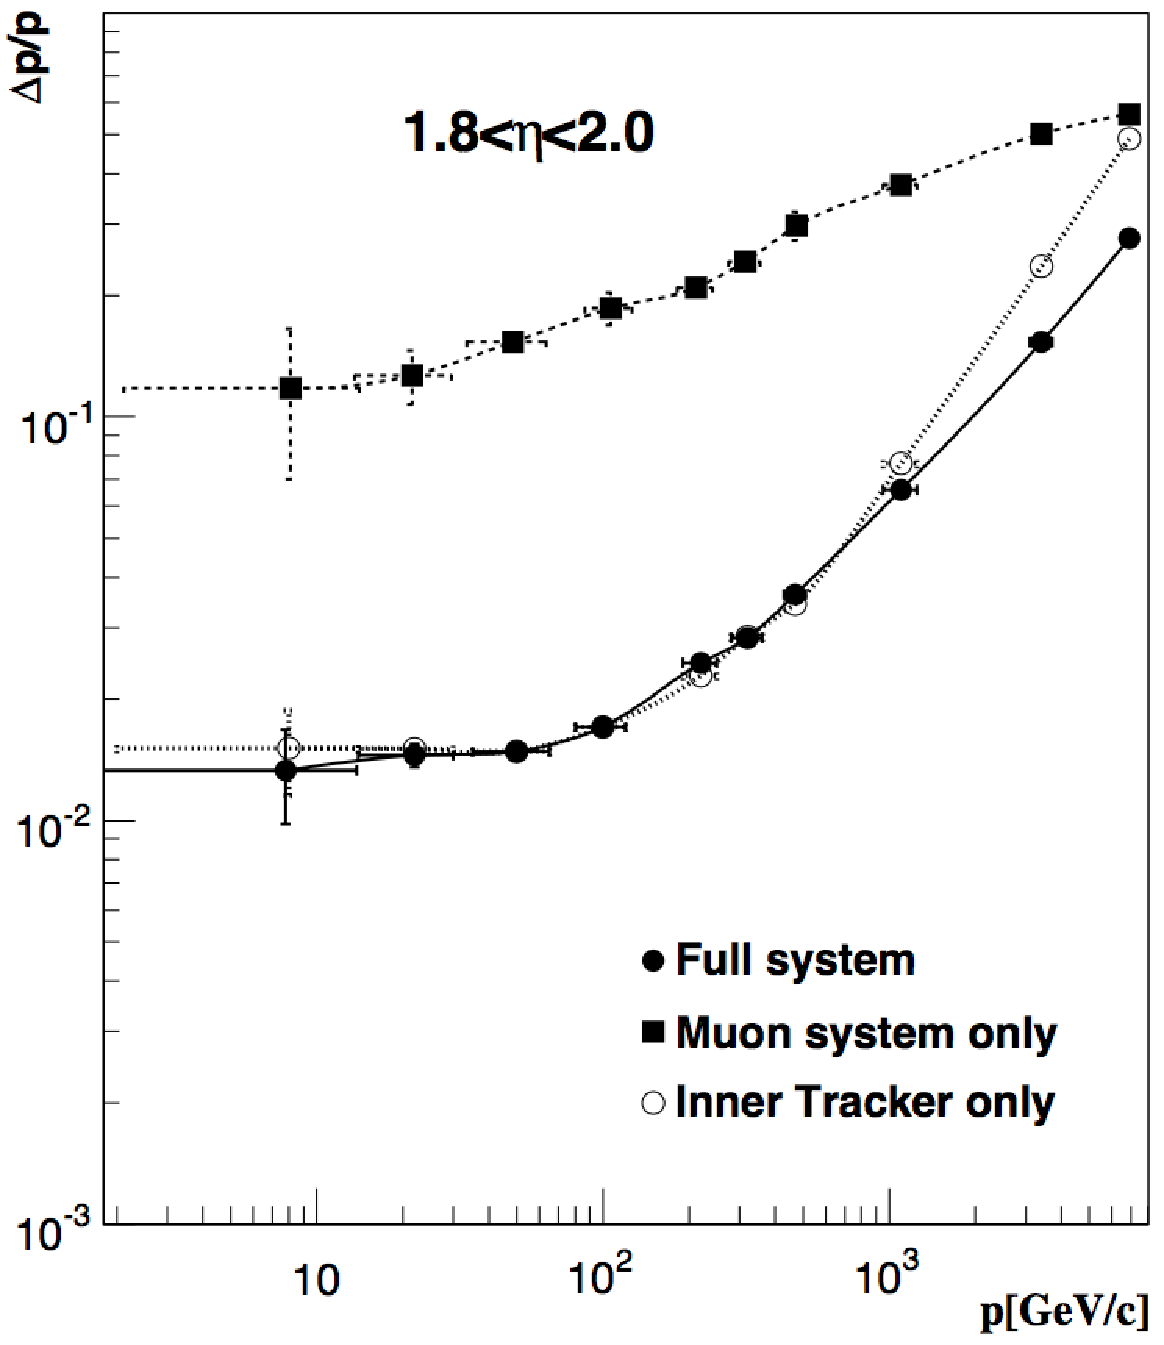
\includegraphics[width=0.45\textwidth]{detector/figs/muonResOuter}
	\caption{Muon momentum resolution as a function of muon momentum using only the inner tracking system, only the muon system, or both combined in the barrel region (left) or endcap region (right).}
	\label{fig:muonSigma}
\end{figure}

Different types of muon detectors are deployed (sometimes in combination) in different sections of the full muon system. In the barrel region ($-1.2<\eta<1.2$) where the muon flux, neutral background, and magnetic field are small, drift tube (DT) chambers are used. In the endcaps where the the muon flux, neutral background, and magnetic field are much greater, cathode strip chambers (CSCs) are used to increase coverage up to $|\eta|<2.4$. In addition to these technologies, both the barrel and endcap systems are supplemented with resistive plate chambers (RPCs) to provide complementary information to the DT and CSC detectors. The layout of the different muon detector components in the barrel and endcap can be seen in figure \ref{fig:muonGeometry}.
 \begin{figure}
	\centering
	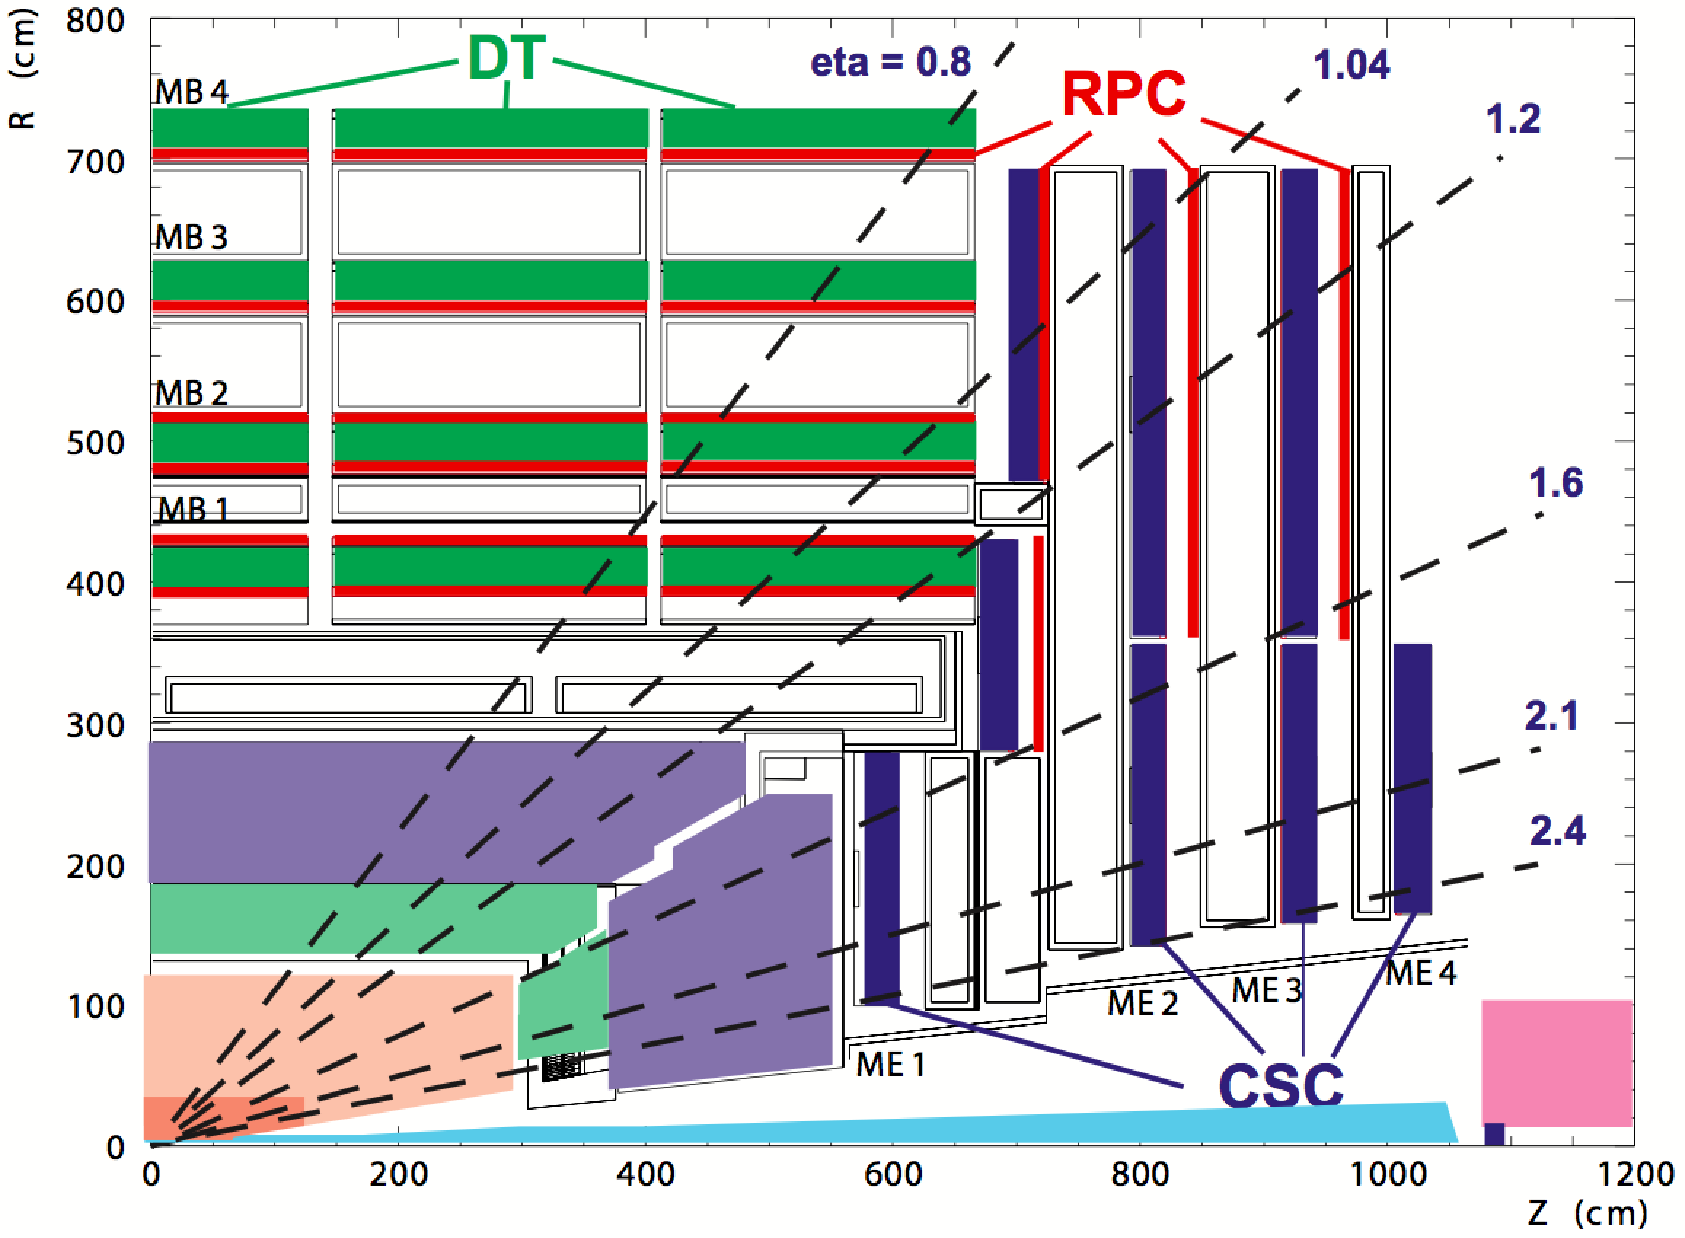
\includegraphics[width=0.75\textwidth]{detector/figs/muonGeometry}
	\caption{Layout of the CMS muon system for initial run configurations. The DT system is used only in the barrel region and CSCs in the endcap region, while RPCs are deployed in both the barrel and endcap.}
	\label{fig:muonGeometry}
\end{figure}

The DT detectors are chambers filled with gas surrounding a wire, with a voltage difference between the wire and outside of the DT. When charged particles pass through the drift chamber, they ionize the gas, and the ionization products will drift across the voltage difference in the tube, resulting in a detectable voltage change in the DT. By measuring both the position along the DT wire where charge is deposited, as well as reconstructing the "drift time" it takes for the ionized particles to reach the wire, DTs provide a 2-dimensional measurement of a particle's position. In CMS, the DT chambers consist of a dozen layers arranged into 3 groups, each with up to 60 DTs. The layers are arranged in such a way that some measure the direction of the muon parallel to the proton beam and others along the perpendicular coordinate, such that the full muon trajectory can be reconstructed by using the DT station information.

The CSCs in each endcap are trapezoidal in shape and overlap in the phi coordinate, increasing the fiducial coverage of the muon system. Each CSC consists of 6 gas gaps, where each gap is comprised of radially aligned cathode strips and a plane of anodes wires nearly perpendicular to the strips. When a muon passes through the CSCs, the ensuing ionization and electron avalanche deposits a charge on the anode wire and an image charge on the cathode strips. A measurement of the muon position can be reconstructed by determining the center-of-gravity of the charge distribution on the cathode strips, and the fast readout of the anode wire is used in low-latency trigger decisions as described in section \ref{subsec:triggers}.

The RPCs are complementary systems in both the barrel and endcap used to improve the time resolution of muon measurements. Each RPC consists of two parallel anode and cathode plates, separated by a gas chamber. The ionization of the gas as muons travel through the chamber is quickly deposited on the plates, and used for a precise time measurement of the muon crossing. Though the spatial resolution of the RPCs is poor, in conjunction with the other muon systems they allow for an unambiguous association of muons with different bunch crossings.
 
\subsection{Trigger Systems}
\label{subsec:triggers}
When operating at design luminosity, the LHC can deliver proton bunches to the collision point at a rate of 40MHz (or 25ns between bunches), resulting in an average collision rate on the order of one billion collisions per second. In order to achieve reasonable rates of data collection for offline storage and processing, the detector must suppress the event rate by six orders of magnitude when selecting events of interest to be saved for physics analyses. This is accomplished through a combination of readout electronics and the trigger systems: the Level-1 trigger (L1) processors and online High-Level triggers (HLT).

The L1 trigger system is comprised of specialized hardware processors to rapidly pre-select events of interest based on the calorimeter and muon systems. Based on the beam crossing frequency, the L1 electronics have only a few microseconds to collect readout data from the front end electronics and execute logic to select events of interest, such that the total time allotted for L1 trigger calculations is $<1\mu s$. During this time the bulk of detector data is held in a buffer while L1 trigger decisions are made based on data with reduced granularity and resolution rapidly collected from the calorimeter and muon systems, where triggers typically check for "trigger primitive" objects (such as photons, muons, electrons, etc.). Trigger primitives must meet certain momentum or energy thresholds, and L1 triggers may also check global data about the event such as the sum of transverse energy or the missing transverse energy (inferred from momentum conservation). 

After an L1 trigger tags an event, high-resolution data is read out from buffers for additional data processing before reaching the HLT. Each event of $\sim1.5MB$ is transferred to front-end readout buffers which then pipes data to a processor containing the HLT code. HLT code is designed to discard events as soon as possible when making trigger decisions and only a subset of objects or partial reconstruction of events may occur before the final trigger decision is made, though HLT algorithms typically approach the quality of final reconstruction. The HLT reduces the L1 output rate to $\mathcal{O}(100\text{Hz})$ for event storage and full reconstruction.
% --------------------------------------------------------------------------- %
% --------------------------------------------------------------------------- %

% --------------------------------------------------------------------------- %
% --------------------------------------------------------------------------- %
\section{CMS Physics Objects}
\label{sec:physicsobjects}

When physics events are fully reconstructed, detector data is used to identify {\it physics objects} representing real particles and event quantities for use in a physics analysis. The physics objects in an event --- such as leptons, jets, or missing energy --- and their properties are used to select events of interest for physics analyses targeting different final states. The properties of physics objects and global event data are also be used to make analysis level decisions of the quality of different objects. Here we describe some of the physics objects referred to in the \mttwo analysis and how they are reconstructed, as well as some global event properties and quality variables used as discriminants for physics objects and events.

\subsection{Particle Flow}
\label{subsec:pf}
Most of the physics objects described in the following sections are reconstructed and identified in CMS using the particle flow (PF) algorithm \cite{Sirunyan:2017ulk}. The PF algorithm is a holistic, iterative algorithm which uses all the available data in the detector to classify "PF candidate" particles in an event. PF works iteratively by identifying tracks and calorimeter deposits into a PF candidate, removing all energy and hits associated with the candidate and repeating the algorithm until all the detector information has been associated to PF objects. First any muon tracks in the inner tracker associated with muon system hits are associated and removed. remaining tracks are extrapolated into the calorimeters, and any energy deposits on the path are associated with the track and removed from further consideration. Once all the tracks have been associated, the remaining energy clusters can be identified with photons and neutral hadrons (depending on their presence in the ECAL or HCAL, respectively). An example of the different tracks and energy deposits associated with various particles can be seen in figure \ref{fig:pfCandidates}.
\begin{figure}
	\centering
	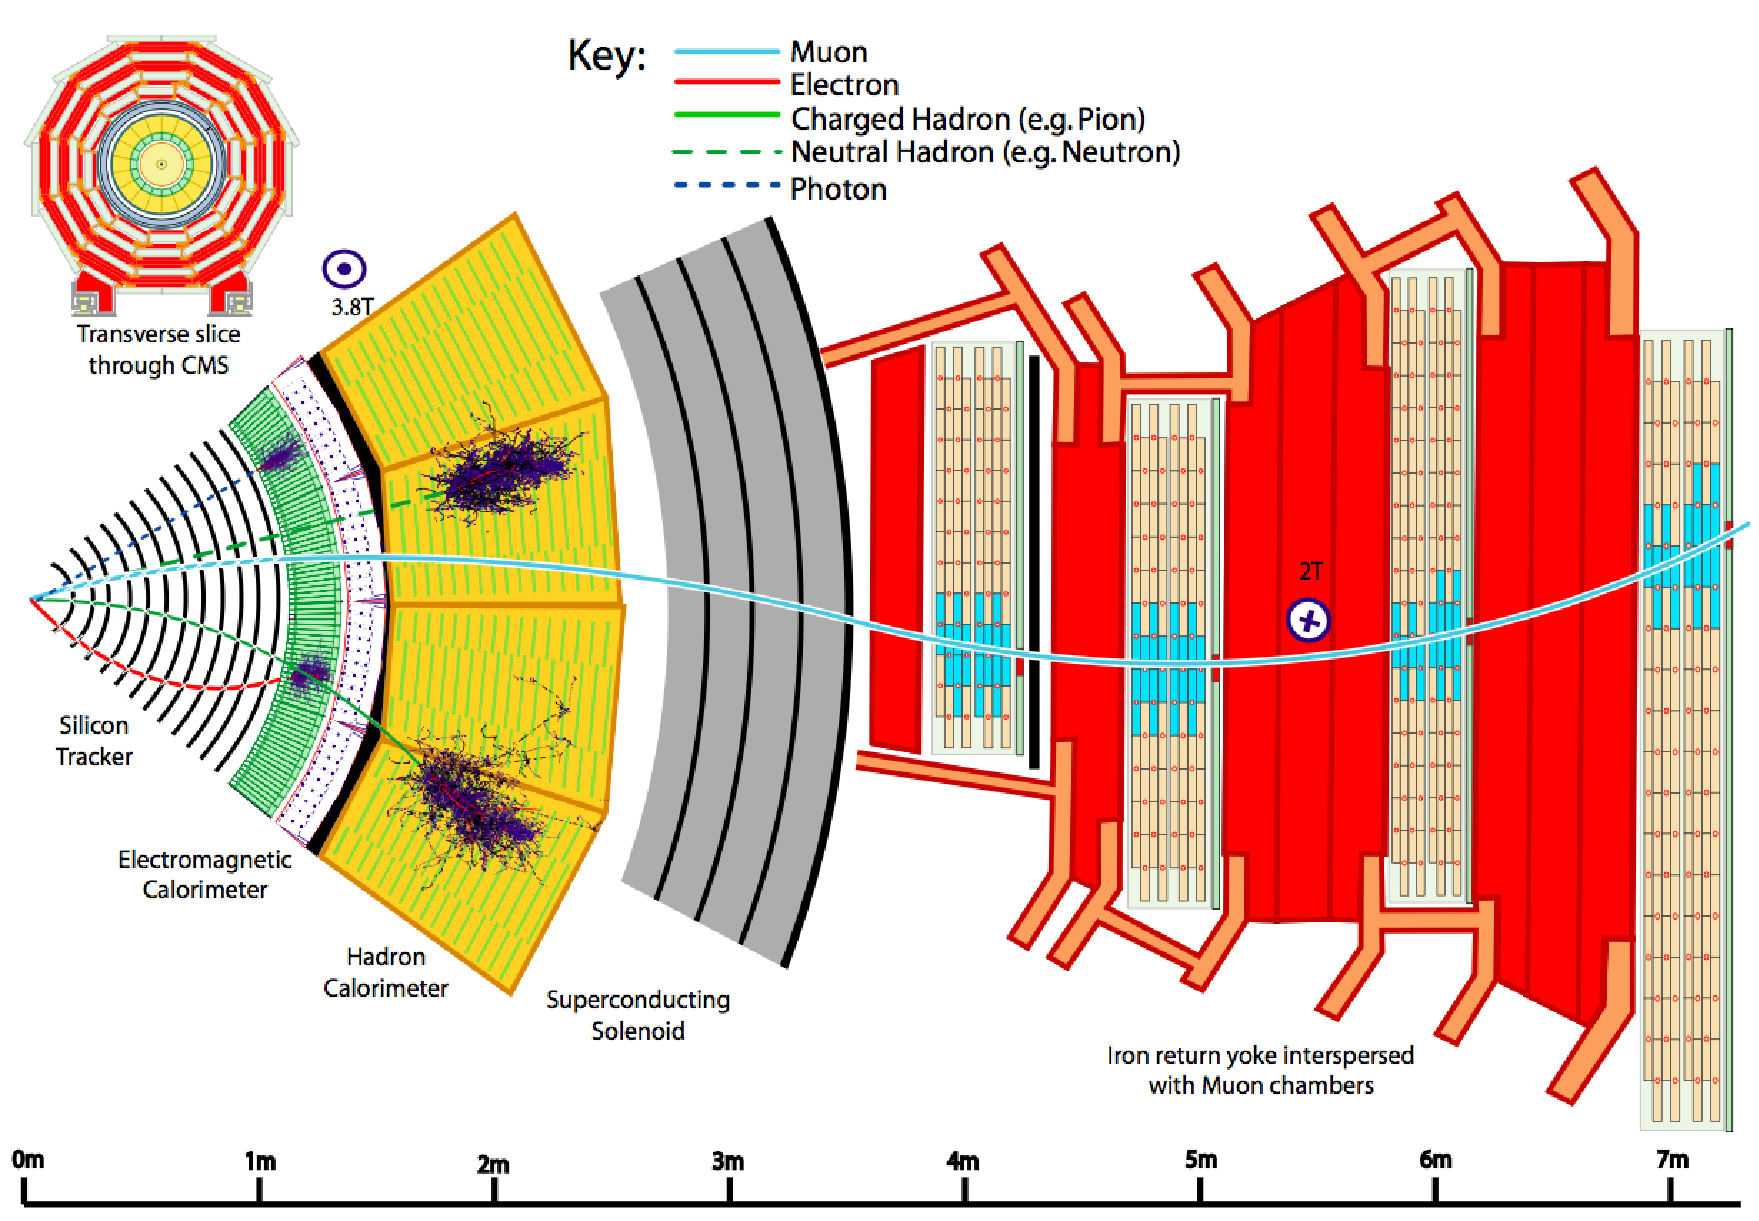
\includegraphics[width=0.95\textwidth]{detector/figs/CMS_Slice_2}
	\caption{A graphic depiction of different particles leaving various signatures in the different CMS detector subsystems. Particles may be detected via tracks hits, energy deposits, or a combination of both.}
	\label{fig:pfCandidates}
\end{figure}

\subsection{Isolation}
\label{subsec:iso}
Isolation is an important distinguishing variable for physics objects measured in the detector. Simply put, isolation measures the total amount of energy in some proximity to a physics object. Because many physics processes results in particle production outside the primary interaction vertex (such as showering, decays, hadronization, pair production, etc.), the isolation of a particle parametrizes the amount of other "activity" surrounding the physics object, and consequently proves a useful discriminant when determining if particles are produced in the primary interaction, or in subsequent physics processes. Particles which are produced in the primary physics process in a collision are sometimes referred to as {\it prompt}, and isolation is a powerful tool in identifying prompt leptons in particular.

\subsection{Electrons, Muons, and Photons}
\label{subsec:lepgamme}
The primary leptons considered in this analysis are electrons and muons (discussed in section \ref{subsec:muons}), and photons are also used as a cross-check in some control regions for background estimates. Prompt electrons and photons are identified in CMS primarily through the use of the ECAL, where they are stopped and deposit all their energy \cite{Baffioni:2006cd,Khachatryan:2015iwa}. Prompt electrons are customarily distinguished by both the presence of a track originating at the primary vertex and a sufficiently low isolation.

Electrons in CMS are identified primarily through the existence of a charged particle track terminating in an energy cluster in the ECAL. As described in section \ref{subsec:ecal}, the ECAL crystals are $\sim25$ radiation lengths deep, and will stop and contain nearly all of the energy of an electron (except perhaps minuscule losses to scattering in the tracker). The charged track leading to the energy deposit distinguishes the charged particle from a neutral particle, and the direction of curvature of the path in the tracker can be used to identify the charge of an electron (or positron).

Photons are distinguished from electrons by the lack of a track in the SVT. As a neutral particle, the only sign of a photon will be the energy deposit in the ECAL where the photon is stopped and deposits all its energy. Photons are typically distinguished from other neutral electromagnetic particles (such as a $\pi^0$) by the shape of the shower in the ecal. Whereas photons typically shower through pair production and bremsstrahlung, other hadronic particles may cascade via different physics processes leading to measurable difference in the shape of the energy cluster.

\subsection{Muons}
\label{subsec:muons}
Prompt muons produced in collisions at the LHC are generally minimum ionizing particles, and will penetrate the bulk of the detector. Without any matching calorimeter deposits, they are reconstructed using hits in the muon system matched to inner tracker hits \cite{Chatrchyan:2009ae}. The muon system flags muon candidates, which are then matched to inner tracker hits for the best fit of the muon track. Given the track hits, the transverse momentum and energy of the muon can be calculated by a fit to the track parameters. As with electrons, muons are customarily distinguished by both the presence of a track originating at the primary vertex and a sufficiently low isolation.

\subsection{Jets}
\label{subsec:jets}
Many particles produced at the LHC are created through the strong interaction, which may produce particles carrying color charge in the final state (i.e. quarks or gluons). Colored particles cannot exist individually due to the phenomenon known as {\it confinement}, and so via the process of {\it hadronization} (also refered to as {\it fragmentation}) they will proliferate in a series of interactions producing additional particle-antiparticle pairs, cascading in a parton shower to form hadronic bound states. When a "bare" quark or gluon is produced in the primary interaction, the ensuing hadronization results in a stream of tightly collimated hadrons aligned with the trajectory of the original bare particle, referred to as a {\it jet}. 

Jets present themselves in CMS as collimated energy deposits in both the ECAL and HCAL, as well as tracks originating at the primary vertex \cite{Schroder:2015czj}. Between the two calorimeters, all the electromagnetic and hadronic components of the jet are stopped and measured by the calorimeters, and any leptons (including muons detected in the muon system) which originate in the cone of the jet are assigned to the total jet energy. The jets are reconstructed using the "anti-k$_T$" algorithm, which clusters jet activity in cones of a fixed radius \cite{Cacciari:2008gp}. The jet is treated as a single physics object with a total energy equal to the sum of its electromagnetic, hadronic, and leptonic components, which by momentum conservation dictates the energy of the prompt quark or gluon that was produced in the primary interaction. 

Furthermore, the substructure of jets and their content can be analyzed to determine the flavor of the parent parton, known as "tagging". Jets are typically tagged to distinguish between those originating from heavy-flavor quarks (bottom or charmed) and light-flavor quarks. Top quarks produced in primary interactions are unique because of their short lifetime. A top quark will decay before hadronization occurs, instead producing a $W$ boson and down-type (down, bottom, or strange) quark which will subsequently hadronize. Searches involving top quarks in the final state typically employ "top-taggers" to search for these signatures of the top quark.

In practice, jets are complicated objects consisting of many constituent particles, and must be clustered and calibrated so that the jet energy closely matches that of the parent parton which produced the jet. Jet energy corrections (JECs) are applied to raw jet energies to compensate for different experimental deviations from the parent parton energy \cite{Khachatryan:2016kdb,CMS-DP-2016-020}. In particular, JECs include corrections to compensate for pileup energy as described in section \ref{subsec:pileup} \cite{Cacciari:2007fd}, detector effects (as a function of $\eta$), energy scale as a function of jet \pt, and residual corrections to account for differences between data and simulation. The JECs are calculated by collecting data events with a Z boson (decaying to electrons or muons) or photon recoiling against a jet. By precisely measuring the bosons energy with the ECAL, scale factors are derived for jets as a function of pseudorapidity $\eta$ and momentum \pt. 

\subsection{Missing Energy}
\label{subsec:met}
Missing energy refers to the sum of all energy which has escaped the detector, and is inferred from a momentum-imbalance in the physics objects measured by the detector \cite{Chatrchyan:2011tn}. Because the momentum of the incident protons is zero perpendicular to the direction of the beam, the momentum of physics objects produced in any collision must sum to zero in the direction transverse to the beamline. The missing transverse energy (\MET), is calculated by taking the negative vector sum of all PF candidates as in equation \ref{eq:met}. \MET is of particular importance to analyses targeting BSM physics, as BSM signatures characteristically contain invisible particles in the final state which escape detection.
\begin{equation}
	\label{eq:met}
	\vec{E}_T^{miss}=-\sum_i^{} \vec{p}_T^{\: i}
\end{equation}

The missing energy in an event is inferred from all other measured quantities in an event, and there are many sources of \MET which are unphysical in nature but rather dependent on experimental effects. Particles from the primary interaction with a sufficiently large pseudorapidity may escape the fiducial region of the detector subsystems, and resolution effects or intrinsic noise in the detector may lead to fluctuations in measured energies. These experimental effects must be suppressed or distinguished from "real" \MET due to physics processes creating particles which escape the detector (e.g. neutrinos). Analyses sensitive to final states with \MET often employ robust data-driven methods to predict or suppress backgrounds which might generate experimental sources of \MET or physics processes which can contribute real \MET (such as \znunu).

\subsection{Monte Carlo Simulation}
\label{subsec:simulation}

Monte Carlo (MC) simulation of events within the CMS detector is frequently generated to understand the expected physics, design analyses, and help predict certain backgrounds. The simulation begins with the underlying physics process of interest, and subsequently models the trajectories of particles in the final state through the detector volume, their interactions in those volumes and with the detector material, the effects of pileup, and the detector response.

The process of generating MC proceeds in multiple steps interfacing different software packages. In this analysis, many MC samples are generated using the POWHEG \cite{Oleari:2010nx} and MadGraph \cite{Alwall:2011uj} generator packages to calculate the matrix elements for the underlying physics process. The calculations performed by these generators are then interfaced with Pythia \cite{Sjostrand:2007gs} to model parton showering and hadronization effects. The material interaction in the detector volume are modeled with the Geant4 toolkit \cite{Agostinelli:2002hh}, and the detector's response is digitized to model the final readout from the event.

Because of the many computationally expensive steps involved in creating MC and the large amount of events required to suppress statistical uncertainties, simulation is occasionally generated with the Fastsim package \cite{1742-6596-331-3-032049} to decrease computational burden at the expense of some modeling quality. When Fastsim is employed in this analysis for the purpose of generating signal MC, effects due to potential mismodeling introduced by the simulation are accounted for in studies of the systematic uncertainty (as shown in section \ref{subsec:signalSyst}).
 
% --------------------------------------------------------------------------- %
% --------------------------------------------------------------------------- %


% --------------------------------------------------------------------------- %
% --------------------------------------------------------------------------- %
